\documentclass[11pt]{article}

%% MinionPro fonts 
%\usepackage[lf]{MinionPro}
%\usepackage{MnSymbol}
\usepackage{microtype}

%% Margins
\usepackage{geometry}
\geometry{verbose,letterpaper,tmargin=1in,bmargin=1in,lmargin=1in,rmargin=1in}

%% Other packages
\usepackage{amsmath}
\usepackage{amsthm}
\usepackage{amsfonts}
\usepackage[shortlabels]{enumitem}
\usepackage{titlesec}
\usepackage{soul}
\usepackage{tikz}
\usepackage{mathtools}
\usepackage{pgfplots}
\usepackage{tikz-3dplot}
\usepackage{algorithmic}
\usepackage[export]{adjustbox}
\usepackage{tcolorbox}
\usepackage{mathrsfs}
\usepackage{multicol}
\usepackage{framed}
\usepackage{optprog}

%% Paragraph style settings
\setlength{\parskip}{\medskipamount}
\setlength{\parindent}{0pt}

%% Change itemize bullets
\renewcommand{\labelitemi}{$\bullet$}
\renewcommand{\labelitemii}{$\circ$}
\renewcommand{\labelitemiii}{$\diamond$}
\renewcommand{\labelitemiv}{$\cdot$}

%% Colors
\definecolor{rred}{RGB}{204,0,0}
\definecolor{ggreen}{RGB}{0,145,0}
\definecolor{yyellow}{RGB}{255,185,0}
\definecolor{bblue}{rgb}{0.2,0.2,0.7}
\definecolor{ggray}{RGB}{190,190,190}
\definecolor{ppurple}{RGB}{160,32,240}
\definecolor{oorange}{RGB}{255,165,0}

%% Shrink section fonts
\titleformat*{\section}{\normalsize\bf}
\titleformat*{\subsection}{\normalsize\bf}
\titleformat*{\subsubsection}{\normalsize\it}

% %% Compress the spacing around section titles
\titlespacing*{\section}{0pt}{1.5ex}{0.75ex}
\titlespacing*{\subsection}{0pt}{1ex}{0.5ex}
\titlespacing*{\subsubsection}{0pt}{1ex}{0.5ex}

%% amsthm settings
\theoremstyle{definition}
\newtheorem{problem}{Problem}
\newtheorem{example}{Example}
\newtheorem*{theorem}{Theorem}
\newtheorem*{bigthm}{Big Theorem}
\newtheorem*{biggerthm}{Bigger Theorem}
\newtheorem*{bigcor1}{Big Corollary 1}
\newtheorem*{bigcor2}{Big Corollary 2}

%% tikz settings
\usetikzlibrary{calc}
\usetikzlibrary{patterns}
\usetikzlibrary{decorations}
\usepgfplotslibrary{polar}

%% algorithmic setup
\algsetup{linenodelimiter=}
\renewcommand{\algorithmiccomment}[1]{\quad// #1}
\renewcommand{\algorithmicrequire}{\emph{Input:}}
\renewcommand{\algorithmicensure}{\emph{Output:}}

%% Answer box macros
%% \answerbox{alignment}{width}{height}
\newcommand{\answerbox}[3]{%
  \fbox{%
    \begin{minipage}[#1]{#2}
      \hfill\vspace{#3}
    \end{minipage}
  }
}

%% \answerboxfull{alignment}{height}
\newcommand{\answerboxfull}[2]{%
  \answerbox{#1}{6.38in}{#2} 
}

%% \answerboxone{alignment}{height} -- for first-level bullet
\newcommand{\answerboxone}[2]{%
  \answerbox{#1}{6.0in}{#2} 
}

%% \answerboxtwo{alignment}{height} -- for second-level bullet
\newcommand{\answerboxtwo}[2]{%
  \answerbox{#1}{5.8in}{#2}
}

%% special boxes
\newcommand{\wordbox}{\answerbox{c}{1.2in}{.7cm}}
\newcommand{\catbox}{\answerbox{c}{.5in}{.7cm}}
\newcommand{\letterbox}{\answerbox{c}{.7cm}{.7cm}}

%% Miscellaneous macros
\newcommand{\tstack}[1]{\begin{multlined}[t] #1 \end{multlined}}
\newcommand{\cstack}[1]{\begin{multlined}[c] #1 \end{multlined}}
\newcommand{\ccite}[1]{\only<presentation>{{\scriptsize\color{gray} #1}}\only<article>{{\small [#1]}}}
\newcommand{\grad}{\nabla}
\newcommand{\ra}{\ensuremath{\rightarrow}~}
\newcommand{\maximize}{\text{maximize}}
\newcommand{\minimize}{\text{minimize}}
\newcommand{\subjectto}{\text{subject to}}
\newcommand{\trans}{\mathsf{T}}
\newcommand{\bb}{\mathbf{b}}
\newcommand{\bx}{\mathbf{x}}
\newcommand{\bc}{\mathbf{c}}
\newcommand{\bd}{\mathbf{d}}

%% LP format
%    \begin{align*}
%      \maximize \quad & \mathbf{c}^{\trans} \mathbf{x}\\
%      \subjectto \quad & A \mathbf{x} = \mathbf{b}\\
%                       & \mathbf{x} \ge \mathbf{0}
%    \end{align*}

%Space between rows:
%\def\arraystretch{2.2}
%
%Space between columns:
%\arraycolsep=1.4pt


%% Redefine maketitle
\makeatletter
\renewcommand{\maketitle}{
  \noindent SA405 -- AMP   \\

  \begin{center}\Large{\textbf{\@title}}\end{center}
}
\makeatother

%% ----- Begin document ----- %%
\begin{document}
  
\title{Lesson 15.  Lagrangian Relaxation}

\maketitle

\section{Motivation}

When talking about branch and bound, we talked about how LP relaxations can be used to give upper bounds on integer programs. Recall that, if $z^*_{IP}$ is the optimal IP solution and $z^*_{LP}$ is the optimal LP solution then:
\[
z^{*}_{IP} \text{ \letterbox~} z^{*}_{LP} \text{ if maximizing}
\]
\[
z^{*}_{IP} \text{ \letterbox~}  z^{*}_{LP} \text{ if minimizing}
\]

Many LP and IP problems have a special structure:
\begin{optprog*}
max & c x \\
st & Ax & = & b \\
   & x & \in & \mathbb{X}
\end{optprog*}

The constraints $x \in \mathbb{X}$ are ``easy'' constraints such as: \vspace{2cm}

The constraints $A x =b$ are ``difficult'' constraints such as: \vspace{2cm}

\textbf{Lagrangian Relaxation} is a method to obtain bounds on integer programs which have this structure. The basic idea of Lagrangian Relaxation is:
	\begin{itemize}
	\item Remove ``hard'' constraints from the problem and place them in the objective function (i.e., relax the IP)
	\item Solve the relaxed problem that now consists of only ``easy'' constraints.
	\end{itemize}
Doing so gives us a bound on the optimal solution.

In many cases, this bound is close to the optimal solution of the original problem. \newpage

\section{Shortest Path Problem with Time Constraints}

\begin{problem}
John is trying to travel from Annapolis to Chicago as cheaply as possible by taking public transportation. Unfortunately, there is no direct route between the two cities, so he will have to travel through some intermediate destinations. The network below shows the cost (in hundreds of dollars) and travel time required for each potential leg of his trip.

\begin{center}
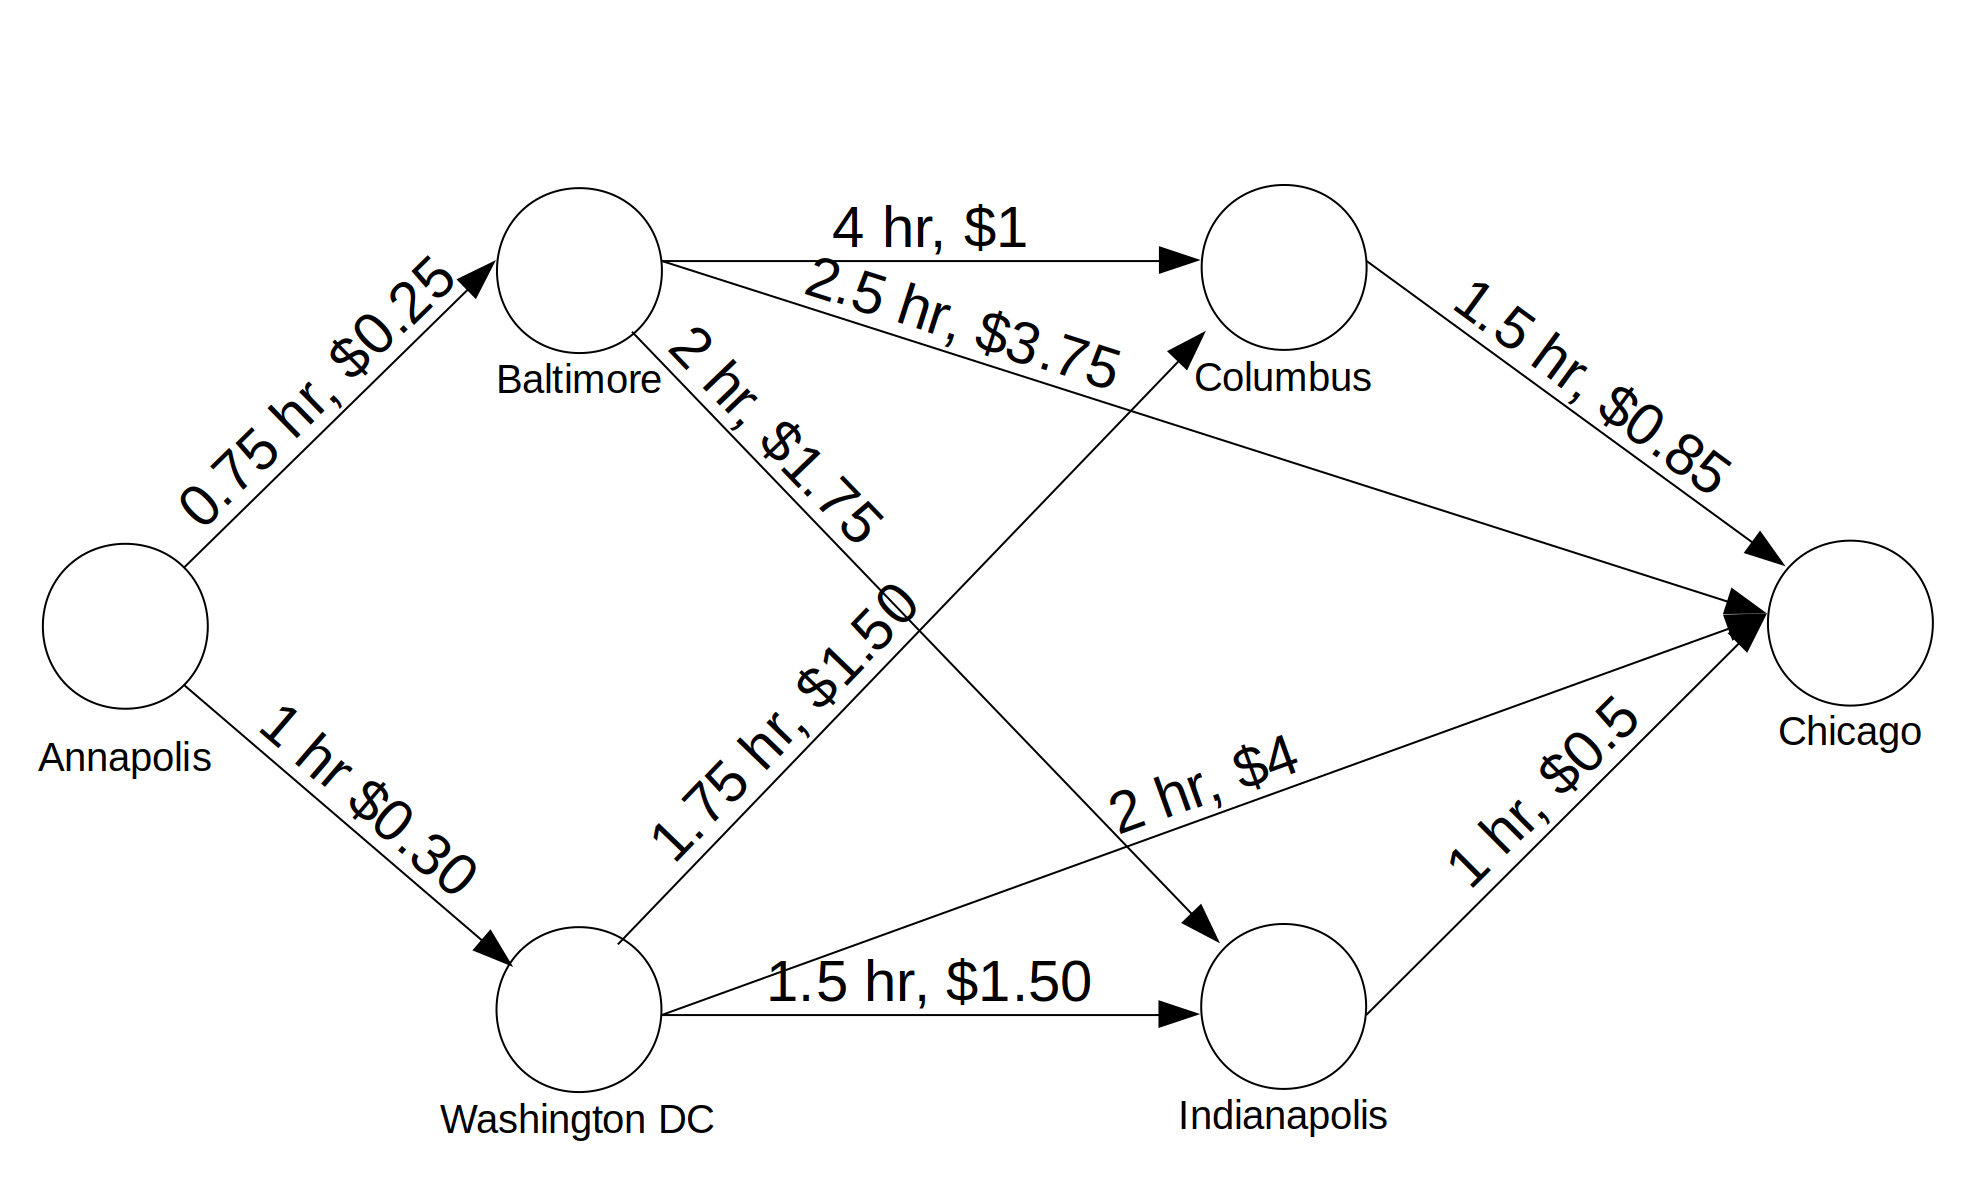
\includegraphics[width=6in]{Short-path.png}
\end{center}

He would like to get to Chicago as quickly as possible on a \$350 budget. He asks you for your help.
\end{problem}

\begin{enumerate}
\item What is the shortest path from Annapolis to Chicago in terms of travel time? Is this path feasible? \vfill
\item What is the shortest path from Annapolis to Chicago in terms of total cost? Is this the shortest path within his budget? \vfill
\end{enumerate}

\newpage

\begin{enumerate}[resume]
\item Using the variables $x_{i,j} = 1$ if edge $(i,j)$ is included in a path, formulate a concrete model that would allow John to minimize his total travel time within his \$350 budget. 
\vfill 
\item Using the usual sets $N$ as the nodes and $E$ as the edges, convert your concrete model into a parameterized model.
\vfill
\newpage

\item In your model, which of your constraints are ``easy'' constraints? Why are they easy? \vspace{1.5cm}
\item In your  model, which of your constraints are ``hard'' constraints? Why are they hard? \vspace{1.5cm}
\end{enumerate}

\section{Lagrangian Relaxation Idea}

A Lagrangian Relaxation is a common method of finding bounds (and sometimes feasible solutions) to solve hard IP problems. They are similar to LP relaxations we use in Branch and Bound.

Recall that to \textbf{relax} a constraint we: \vspace{1cm}

In an LP relaxation, the \wordbox constraints of the IP are relaxed.

In a Lagrangian relaxation, the \wordbox constraints of the IP are relaxed.

\begin{tcolorbox}
Lagrangian relaxation:
For an IP of the form:
\begin{optprog*}
min & c x \\
st & Ax & \leq & b \\
   & x & \in & \mathbb{X}
\end{optprog*}
Where $x \in \mathbb{X}$ are easy constraints and $A x \leq b$ are hard constraints
	\begin{enumerate}
	\item Select a penalty $\lambda \geq 0$ to ``pay'' if the hard constraints are violated.
	\item Relax the constraints from the feasible region and instead put them in the objective function multiplied by the penalty. That is, your objective function becomes:
	\[
	\text{min } c x + \lambda (Ax - b)
	\]
	\end{enumerate}
\end{tcolorbox}

\begin{problem}
Write the Lagrangian Relaxation of your parameterized IP problem for any value of $\lambda$.
\end{problem}
\newpage

\section{Properties of Lagrangian Relaxation}

Let $z^*(\lambda)$ be the optimal objective function value of the Lagrangian Relaxation. Let's think about what happens for various values of $\lambda$:
\begin{itemize}
\item If $\lambda = 0$ what solution is found? \vfill

Then, $z^*(\lambda) \letterbox~ z^*_{IP}$
\item As $\lambda$ increases from 0, what happens? \vfill

Thus, $z^*(\lambda) \letterbox~ z^*_{IP}$ for \textbf{any value of} $\lambda$
\end{itemize}

This is the key property of Lagrangian relaxation!

\begin{tcolorbox}
In general, for a maximization problem:

\[
z^*(\lambda) \geq z^*_{IP}
\]
 
For a minimization problem:
\[
z^*(\lambda) \leq z^*_{IP}
\]

For all values of $\lambda \geq 0$

\end{tcolorbox}

\newpage

\begin{problem}
Let's see an example, suppose $\lambda = 1$.

\begin{center}
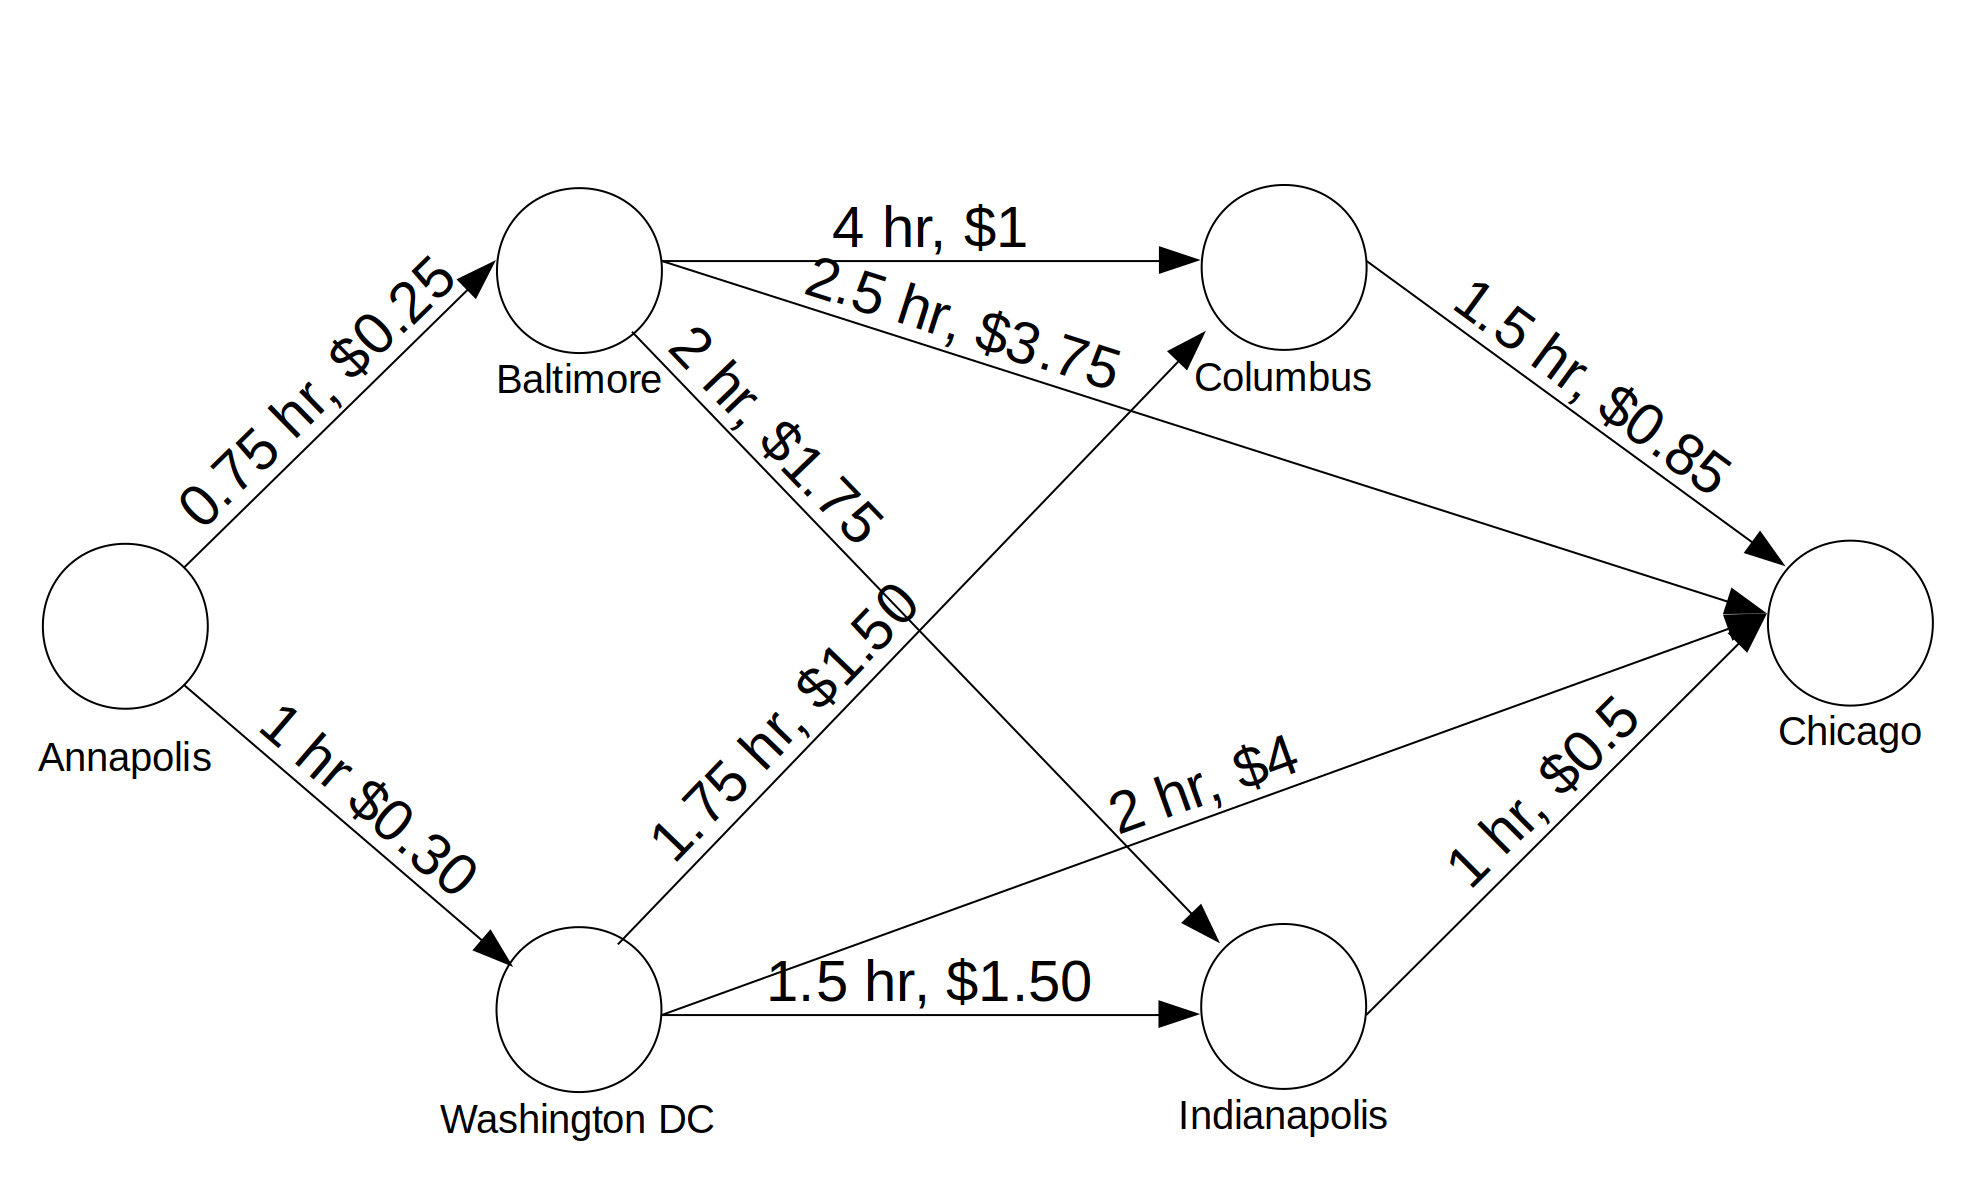
\includegraphics[width=6in]{Short-path.png}
\end{center}
\end{problem}
\begin{enumerate}
\item What is the shortest path in this network? \vfill
\item Is this solution feasible to the original problem? \vfill
\item What is the objective function value of this solution in the original problem? \vfill
\item What is the objective function value of this solution in the Lagrangian Relaxation? \vfill
\end{enumerate}

\newpage


Since the Lagrangian relaxation is an upper bound for any value of $\lambda$, a related problem is to find the optimal $\lambda$ to find the best bound. In this case we should be trying to find as \wordbox of a bound as possible.

\vspace{2cm}

Mathematically, this is called the \textbf{Lagrangian Dual} problem.

\vfill

\section{Other Considerations}

\begin{itemize}
\item There are equivalent cases of Lagrangian relaxation for equality and $\geq$ constraints; usually all that changes is a sign in the objective function.
\item There are cases where the Lagrangian Relaxation provides an exact bound to the optimal solution of the IP. This makes it a very powerful tool.
\item Some problems are so hard to solve; the best we can do it compute bounds on the optimal solution. Lagrangian Relaxation is a good tool for this.
\end{itemize}

%%%

\end{document}


